\documentclass[a4paper,10pt]{article}

\usepackage[top=0.38in, bottom=0.35in, left=0.45in, right=0.45in]{geometry}
\usepackage{mathptmx}
\usepackage[T1]{fontenc}
\usepackage{titlesec}
\usepackage{enumitem}
\usepackage{hyperref}
\usepackage{xcolor}
\usepackage{graphicx}
\usepackage{tikz}

% Color Definitions
\definecolor{primary}{RGB}{20, 50, 95}
\definecolor{darkgray}{RGB}{45, 45, 45}
\definecolor{accent}{RGB}{0, 80, 165}

% Hyperlink Setup
\hypersetup{
    colorlinks=true,
    linkcolor=accent,
    urlcolor=accent,
    pdfauthor={Anshika Keshari},
    pdftitle={Anshika Keshari - Resume}
}

% Page Style Setup
\pagestyle{empty}
\urlstyle{same}

% Section Title Formatting
\titleformat{\section}
  {\large\bfseries\color{primary}}
  {}
  {0pt}
  {}
  [\vspace{1.5pt}\hrule height 0.5pt\vspace{3pt}]

\titlespacing*{\section}{0pt}{5.5pt}{2.5pt}

% Custom Itemize List Formatting
\setlist[itemize]{leftmargin=12pt, topsep=1.0pt, itemsep=1.5pt, parsep=0pt}

\begin{document}

%----------------------------------------------------------------------------------------
%   HEADER
%----------------------------------------------------------------------------------------
\noindent
\begin{minipage}[c]{0.78\textwidth}
    {\LARGE \bfseries \color{primary} ANSHIKA KESHARI}\\[3.5pt]
    {\small
    Bhubaneswar, Odisha -- 751024 \\[2pt]
    \href{mailto:anshikakeshari0@gmail.com}{anshikakeshari0@gmail.com} \ $|$ \ +91-7869009573 \\[2pt]
    \href{https://linkedin.com/in/anshika-keshari-7925bb3aa}{linkedin.com/in/anshika-keshari-7925bb3aa} \ $|$ \ \href{https://github.com/anshika-keshari24}{github.com/anshika-keshari24}
    }
\end{minipage}%
\hfill
\begin{minipage}[c]{0.20\textwidth}
    \raggedleft
    \begin{tikzpicture}
        \begin{scope}
            \clip [rounded corners=4pt] (0,0) rectangle (2.10cm, 2.60cm);
            \node[inner sep=0pt] at (1.05cm, 1.25cm) {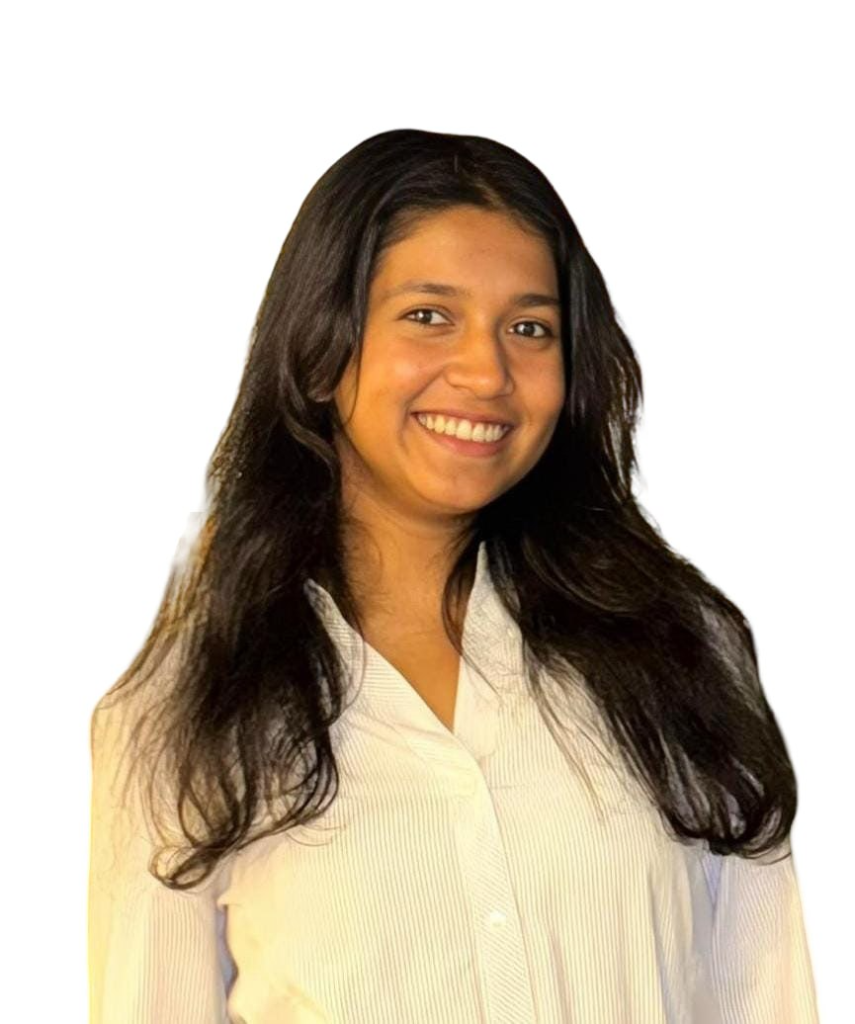
\includegraphics[width=2.70cm]{profile_photo.png}};
        \end{scope}
        \draw[black!60, line width=0.5pt, rounded corners=4pt] (0,0) rectangle (2.10cm, 2.60cm);
    \end{tikzpicture}
\end{minipage}

\vspace{2pt}

%----------------------------------------------------------------------------------------
%   EDUCATION
%----------------------------------------------------------------------------------------
\section{Education}
\noindent\textbf{Kalinga Institute of Industrial Technology (KIIT)} -- \textit{B.Tech, Computer Science \& Engineering} \ $|$ \ \textbf{CGPA: 8.32} \hfill \textit{2023 -- 2027} \\[1.8pt]
\textbf{Gurukul Public School}, Kawardha -- \textit{CBSE Class XII (Science Stream), 2023} \ $|$ \ \textit{Class X, 2021}

%----------------------------------------------------------------------------------------
%   EXPERIENCE
%----------------------------------------------------------------------------------------
\section{Experience}
\noindent\textbf{Research Intern -- Cybersecurity \& Cyber Resilience} \hfill \textit{May 2026 -- Jul 2026} \\
\textit{Dr. SPM International Institute of Information Technology (IIIT Naya Raipur)} \hfill \textit{Raipur, Chhattisgarh}
\begin{itemize}
    \item \textbf{INTPART ResCri Project}: Contributing to the \textbf{India--Norway collaborative research project} between IIIT Naya Raipur and Norwegian research institutions on cyber resilience for critical infrastructure using Digital Twins.
    \item \textbf{Graph Digital Twin Architecture}: Engineered a \textbf{Graph Digital Twin (GDT)} framework combining Graph Neural Networks (\textbf{GraphSAGE, GNNs}) for real-time anomaly detection and cyber-attack classification.
    \item \textbf{Explainable AI (XAI) \& Automation}: Integrated \textbf{GNNExplainer} and \textbf{Integrated Gradients} for node/edge attribution, powering sub-15ms automated cyber-physical attack mitigation.
\end{itemize}

%----------------------------------------------------------------------------------------
%   KEY PROJECTS
%----------------------------------------------------------------------------------------
\section{Key Projects}

\noindent\textbf{Graph Digital Twin for Cyber Resilience} \hfill \textit{Python, PyTorch, Pandapower, NetworkX}
\begin{itemize}
    \item Engineered a simulation testbed to analyze how sensor data tampering impacts interconnected power grid substations.
    \item Implemented Python scripts to process live sensor telemetry and benchmark machine learning models on anomaly detection.
\end{itemize}

\vspace{2.5pt}
\noindent\textbf{Anti-Money Laundering (AML) Detection System} \hfill \textit{Python, Random Forest, XGBoost, Scikit-learn, Pandas}
\begin{itemize}
    \item Fraud Detection using Graph Analytics, Explainable AI, and Privacy-Preserving Techniques
    \item Designed a machine learning pipeline to detect money laundering in financial transactions using Random Forest with SMOTE for class imbalance, SHAP for explainability, and an interactive dashboard for real-time risk analysis.
\end{itemize}

\vspace{2.5pt}
\noindent\textbf{Real-Time Threat Monitoring Dashboard} \hfill \textit{Python, Flask, JavaScript, Chart.js, Scikit-learn}
\begin{itemize}
    \item Built a full-stack web dashboard with a Flask REST API serving anomaly scores from the Graph Digital Twin and AML models to a JavaScript front end.
    \item Visualized live grid-sensor telemetry and flagged high-risk transactions using interactive Chart.js graphs and color-coded alerts.
    \item Added filters by substation, time window and risk level so analysts can quickly investigate suspicious activity.
\end{itemize}

%----------------------------------------------------------------------------------------
%   SKILLS & COMPETENCIES
%----------------------------------------------------------------------------------------
\section{Skills \& Competencies}
\begin{itemize}
    \item \textbf{Languages}: Java, Python, JavaScript, SQL, PowerShell, LaTeX
    \item \textbf{AI / ML \& Security}: Scikit-learn, XGBoost, Random Forest, PyTorch (Basics), Pandas, NumPy, OpenCV, NLP, Graph Neural Networks (GNNs)
    \item \textbf{Tools \& Databases}: Git, GitHub, VS Code, Linux (Ubuntu), AWS, MySQL, Flask, REST APIs, Chart.js, Relational DBMS
    \item \textbf{CS Fundamentals}: Data Structures \& Algorithms, Operating Systems, OOP (Java), DBMS, Computer Networks
    \item \textbf{Soft Skills}: Problem Solving, Technical Communication, Analytical Thinking, Self-Learning
\end{itemize}

%----------------------------------------------------------------------------------------
%   CERTIFICATIONS
%----------------------------------------------------------------------------------------
\section{Certifications}
\begin{itemize}
    \item \textbf{8-Week Summer Training Certificate in AI/ML \& Cybersecurity} -- KIIT (Jul 2026)
    \item \textbf{Data Engineering} -- ExcelR (Jun 2026) \ $|$ \ \textbf{Corporate Governance} -- Coursera \ $|$ \ \textbf{Corporate Responsibility} -- London Business School (2026)
\end{itemize}

%----------------------------------------------------------------------------------------
%   EXTRA CURRICULAR ACTIVITIES & LEADERSHIP
%----------------------------------------------------------------------------------------
\section{Extra Curricular Activities \& Leadership}
\begin{itemize}
    \item \textbf{Leadership}: Team Lead, Kzarshion (Krystal Fashion Society), KIIT -- led 100+ members and coordinated events; Head Girl, Gurukul Public School (2022--23) -- represented 1,000+ students.
    \item \textbf{Fashion}: \textbf{1st Position}, Melange'26 Fashion Show, KIITfest 2026; \textbf{Runner-Up}, National Group Fashion Showcase, IIT Guwahati.
    \item \textbf{Arts}: Completed \textbf{6-Year Diploma in Kathak Classical Dance}, demonstrating artistic discipline.
\end{itemize}

\end{document}
